%!TEX program = xelatex
% !Mode:: "TeX:UTF-8"
%% 请使用 XeLaTeX 编译本文.
\documentclass[smd,entitle,forlib,AutoFakeBold]{NJTECHMaster}   
% 选项 smd: Specialist Master's Degree, 产生专业硕士学位论文封面、页眉.
% 选项 forprint: 交付打印时, 建议加上此选项,会自动增加空白页保证每个章节为奇数页, 消除彩色链接文字, 避免彩色字迹打印偏淡.
% 选项 forlib: 提交给图书馆的电子版(盲审也交这个版本), 需要加上选项 forlib, 以消除空白页和彩色链接.
% 选项 entitle: 使下文的\spine选项生效,尽量不要在中文标题中带英文,对齐还有点小问题.
% 选项AutoFakeBold:避免在Windows下加粗的宋体变成黑体,Mac下可不加该选项
%%%=== 参考文献=== %%%
\bibliographystyle{gbt7714}        % 外挂的满足gbt7714的参考文献样式

%%%%%%%%%%%%%%%%%%%%%%%%%%%%%%%%%%%%%%%%%%%%%%%%%

\begin{document}
	%%%%%%%-------------------------------------------------
	\fenleihao{}  % 分类号:《中国图书资料分类法》的类号
	\miji{}                % 密级
	\UDC{}               %《国际十进制分类法UDC》的类号
	\bianhao{}  % 学校编号, 10291是南京工业大学的编号
	
	\title{南京工业大学硕士论文~\LaTeX~模板}
	\spine{南京工业大学硕士论文 ~ \rotatebox[origin=c]{-90}{~\LaTeX{}~} 模板}%边栏的书脊,手动将英文字母填在rotatebox里,不启用entitle选项时可忽略
	\Etitle{A \LaTeX~Thesis Template for NanjingTech University} % 英文题目
	\author{郭索眸}%作者姓名
	\Eauthor{Suomou Guo}            %作者英文名
	\Csupervisor{白光伟\quad 顾慎凯}        %指导教师中文名,单导师时使用可使用“赵志宏\quad 教授”
	\Esupervisor{Prof.~Guangwei Bai \\and\\Lecturer.~Shenkai Gu}     %指导教师英文名、职称,单导师时使用"Prof.~Zhihong Zhao"
	\Cmajor{计算机技术}                          % 一级专业中文名[ SMD:领域名称]
	\Cspeciality{工程硕士}                     % 二级学科名称[ SMD:工程硕士]
	
	\date{2022年4月}                    % 硕士类只写年月. 要注意和英文日期一致!!
	\Edate{April 2022}                   % 英文封面日期
	
	%-----------------------------------------------------------------------------
	%\pdfbookmark[0]{封面}{title}         % 封面页加到 pdf 书签
	\maketitle
	%-----------------------------------------------------------------------------
	% !Mode:: "TeX:UTF-8"

%%% 此部分包含: (1) 英文封面 (无需改动) ; (2) 郑重声明 (无需改动) ; (3)项目资助(需要自己填写) .

%%%%%%%%%%%%%%%%%%%%%%%%%%%%%
%%% -------------  英文封面 (无需改动)-------------   %%%
%%%%%%%%%%%%%%%%%%%%%%%%%%%%%
\thispagestyle{empty}
\renewcommand{\baselinestretch}{1.5}  %下文的行距
\vspace*{0.5cm}
\setmainfont{Times New Roman}

\begin{center}{\zihao{3} \textbf{\MakeUppercase{\the\Etitle}} \par}\end{center}

\vspace*{25mm} %插入空白
%\vfill

\begin{center}
\zihao{3}
A Thesis Submitted to\\
Nanjing Tech University\\
For the Professional Degree of Master of\\
Engineering\\

\vspace*{20mm} %插入空白

By\\
{\sc \the\Eauthor}      \\

\vspace*{20mm} %插入空白

Supervised by\\
{\sc \the\Esupervisor}\\


\vspace*{25mm} %插入空白

\the\Edate

\end{center}
%%%%%%%--判断是否需要空白页-----------------------------
  \iflib
  \else
  \newpage
  \thispagestyle{empty}
  \cleardoublepage
  \fi
  
  
%%%%%%%-------------------------------------------------
%%%--- 加入``郑重声明'' --- %%%%%%%%%%%%%%%%%
{
	\pagestyle{empty}
	\newpage
	%\setlength{\parindent}{0pt} %
	\vspace*{20pt}
	\begin{center}{\zihao{3}\songti \textbf{学位论文独创性声明}}\end{center}
	\par\vspace*{30pt}
	\renewcommand{\baselinestretch}{2}
	{\zihao{-4} \songti %
		
		
		\noindent 本人声明所呈交的学位论文是我个人在导师指导下进行的研究工作及取得的研究成果。尽我所知,除了文中特别加以标注和致谢的地方外,论文中不包含其他人已经发表或撰写过的研究成果,也不包含为获得南京工业大学或其它教育机构的学位或证书而使用过的材料。与我一同工作的同志对本研究所做的任何贡献均已在论文中作了明确的说明并表示了谢意。\\
		\begin{tabular}{lp{3cm}p{0cm}lp{3cm}l}
			\raisebox{-0.5ex}[0pt]{\makebox[2.5cm][s]{研\hfill 究\hfill \hfill 生\hfill 签\hfill 名:}} & {}\hfill\raisebox{-0.5ex}[0pt]{}\hfill{} &  &
			\raisebox{-0.5ex}[0pt]{\makebox[2.5cm][s]{日\hfill 期:}} & {}\hfill\raisebox{-0.5ex}[0pt]{}\hfill{} & \\\cline{2-2}\cline{5-5}
		\end{tabular}
		
		
		\vskip2cm
		\par
	}
	
	\begin{center}{\zihao{3}\songti \textbf{学位论文的使用声明}}\end{center}
	\par\vspace*{30pt}
	\renewcommand{\baselinestretch}{2}
	{\zihao{-4} \songti %
		
		
		{\zihao{-1} \noindent $ \square  $}{\zihao{-2} \noindent 1、}南京工业大学、国家图书馆、中国科学技术信息研究所、万方数据电子出版社、中国学术期刊(光盘版)电子杂志社有权保留本人所送交学位论文的复印件和电子文档,可以采用影印、缩印或其他复制手段保存论文并通过网络向社会提供信息服务。论文的公布(包括刊登)授权南京工业大学研究生部办理。(打钩生效)\\
		{\zihao{-1} \noindent $ \square  $}{\zihao{-2}  2、}本论文已经通过保密申请,请保留三年后按照第一项公开(打钩生效)\\
		{\zihao{-1} \noindent $ \square  $}{\zihao{-2}  3、}本论文已经通过校军工保密申请,不予公开(打钩生效)\\
		\begin{tabular}{lp{3cm}p{0cm}lp{3cm}l}
			\raisebox{-0.5ex}[0pt]{\makebox[2.5cm][s]{研\hfill 究\hfill \hfill 生\hfill 签\hfill 名:}} & {}\hfill\raisebox{-0.5ex}[0pt]{}\hfill{} &  &
			\raisebox{-0.5ex}[0pt]{\makebox[2.5cm][s]{导\hfill 师\hfill 签\hfill 名\hfill :}} & {}\hfill\raisebox{-0.5ex}[0pt]{}\hfill{} & \\\cline{2-2}\cline{5-5}
			\raisebox{-0.5ex}[0pt]{\makebox[2.5cm][s]{日\hfill 期:}} & {}\hfill\raisebox{-0.5ex}[0pt]{}\hfill{} &  &
			\raisebox{-0.5ex}[0pt]{\makebox[2.5cm][s]{日\hfill 期:}} & {}\hfill\raisebox{-0.5ex}[0pt]{}\hfill{} & \\\cline{2-2}\cline{5-5}
		\end{tabular}
	
	%%%%%%%-------------------------------------------------
	%%%--- 加入``项目资助'' --- %%%%%%%%%%%%%%%%%
		\clearpage
		\vspace*{20pt}
		\vfill
		\noindent 本文工作得到以下项目资助:
		\begin{enumerate}[1. ]
			\item 国家自然科学基金项目“链路相关无线网络中基于网络编码的数据分发机制研究”(项目编号:61502230);
			\item 江苏省自然科学基金项目“面向无线数据分发应用的新型网络编码机制研究”(项目编号:BK20150960);
		\end{enumerate}
		
	
	
	%%%%%%%--判断是否需要空白页-----------------------------
	\iflib
	\else
	\newpage
	\cleardoublepage
	\fi
	%%%%%%%-------------------------------------------------
}

\renewcommand{\baselinestretch}{1.6}
\small\normalsize




    % 加入英文封面、独创性声明、使用声明、项目资助情况
	\frontmatter
	\pagenumbering{Roman}               % 正文之前的页码用大写罗马字母编号.
	
	\cleardoublepage
	\newpage  
	\pagestyle{fancy} \fancyfancy
	%------------------------------------------------------------------------------
	\renewcommand{\baselinestretch}{1.7} \normalsize %行距
	% !Mode:: "TeX:UTF-8"

%%% 说明: 此部分需要自己填写的内容:  (1) 中文摘要及关键词 (2) 英文摘要及关键词

%%%%%%%%%%%%%%%%%%%%%%%
%%% ------------ 中文摘要 ---------------%%%
%%%%%%%%%%%%%%%%%%%%%%%
\begin{cnabstract}
	
\thispagestyle{onlytitle}

本文主要介绍和讨论了南京工业大学硕士毕业论文的~\LaTeX~模板.
指明了编译方法, 强调了公式排版的一些细节问题, 也指出了一些常见的排版错误.



\end{cnabstract}

\vspace*{10mm} %插入空白

%%%--------- 关键词 -------- %%%
\cnkeywords{毕业论文 \qquad \LaTeX{}\qquad 模板\qquad XeLaTeX }

%%%%%%%%%%%%%%%%%%%%%%%


%%%%%%%%%%%%%%%%%%%%%%%
%%% ------------ 英文摘要 ---------------%%%
%%%%%%%%%%%%%%%%%%%%%%%
\begin{enabstract}
\thispagestyle{onlytitle}
This thesis is a study on the theory of \dots.




\end{enabstract}
\vspace*{10mm} %插入空白
%%%------ 英文关键词 ------- %%%
\enkeywords{Graduation thesis;\LaTeX{};Template;XeLaTeX}


      % 加入中英文摘要.
	%---把目录加入到书签---%%%%%%%%%%%%%%
	%\pdfbookmark[0]{目录}{toc}%%%%%%%%%%%%
	\tableofcontents
	\thispagestyle{toc}
	\addcontentsline{toc}{chapter}{目\texorpdfstring{\quad}{} 录}
	%------------------------------------------------------------------------------
	\mainmatter %% 重新计算页码,以下是正文
	%%%%%%%%%%%%%%%%%%%%%%%%%%%%%%%%%%%%
	\renewcommand{\arraystretch}{1.5}%表格行间距
	
\chapter{绪论}
\section{具体使用步骤}

\begin{description}
	
	\item[Step 1]  进入 includefile 文件夹,  打开frontmatter.tex,  midmatter.tex,  backmatter.tex 这三个文档,
	分别填写 (1) 项目资助,(2)中文摘要、英文摘要, (3) 科研项目、学术成果、奖项、致谢。
	
	\item[Step 2]  打开主文档 MasterTemplate.tex, 填写题目、作者等等信息, 书写正文。
	
	\item[Step 3]  使用 XeLaTeX 编译. 具体见 \ref{sec-compile} 节。
	
	
\end{description}

\section{编译的方法}\label{sec-compile}

默认使用 XeLaTeX 编译, 直接生成~pdf 文件。

若另存为新文档, 请确保文档保存类型为 \verb|:UTF-8|。当然目前很多编辑器默认文字编码为 UTF-8。
WinEdt 9.0 之后的版本都是默认保存为 UTF-8 的。

\section{文档类型选择}
文档类型包括一下几类选项:

% Please add the following required packages to your document preamble:
% \usepackage{multirow}
\begin{table}[h]
	\centering
	\caption{文档类型选项}
	%英文标题begin
	\addtocounter{table}{-1}
	%\SetEnglishCaption
	\renewcommand{\tablename}{Table}
	\caption{Document type options}
	\renewcommand{\tablename}{表}
	%英文标题end
	\label{tbl-DTO}
	\vspace{2pt}
	\small
	\begin{tabular}{l|l|l}
		\hline
		\multicolumn{1}{c|}{选项组}                   & 选项           & 含义                                                                                                                                                                                                                                                                                      \\ \hline
		\multicolumn{1}{c|}{\multirow{2}{*}{论文类型}} & 留空           & 学术学位                                                                                                                                                                                                                                                                                    \\ \cline{2-3} 
		\multicolumn{1}{c|}{}                      & smd          & 专业学位                                                                                                                                                                                                                                                                                    \\ \hline
		\multirow{3}{*}{输出类型}                       & 留空           & 链接会加彩色框便于确认,会自动增加空白页保证每个章节为奇数页                                                                                                                                                                                                                                                          \\ \cline{2-3} 
		& forprint     & 消除彩色链接,自动增加空白页保证每个章节为奇数页                                                                                                                                                                                                                                                    \\ \cline{2-3} 
		& forlib     & 消除了空白页和彩色链接,提交给图书馆(以及盲审)时使用这个版本                                                                                                                                                                                                                                                         \\ \hline
		英文标题                                        & entitle      & 使~\verb|\spine{}|~生效,非中文字符内容填写在~\verb|\rotatebox[origin=c]{-90}{}|~中 \\ \hline
		字体修正                                        & AutoFakeBold & 避免在Windows下加粗的宋体变成黑体,Mac下可不加该选项                                                                                                                                                                                                                                                         \\ \hline
	\end{tabular}
\end{table}

例如,学术硕士论文,中文标题中含义英文字符,在Mac上输出打印版本:\\ \verb|\documentclass[forprint]{NJTECHMaster}|

专业硕士论文,纯中文标题,在Windows上输出图书馆提交版本:\\	\verb|\documentclass[smd,forlib,AutoFakeBold]{NJTECHMaster} | 
 
相关解释见接下来的两节.

\section{打印的问题}
\begin{enumerate}[i)]
	\item  硕士论文要求\colorbox{yellow}{双面打印}.
	\item  关于文档选项 forprint: 交付打印时, 建议加上选项 forprint, 以消除彩色链接文字, 避免打印字迹偏淡。同时该选项已经添加好了空白页(该页显示效果为完全空白但计算了页码)使得每章在奇数页起始(即装订后翻开在右手边那页)。
	\item  打印时留意不要缩小页面或居中. 即页面放缩方式应该是``无''或者``100\%'' (Adobe Reader XI 是选择``实际大小'')。
	有可能页面放缩方式默认为``适合可打印区域'', 会导致打印为原页面大小的 $97\%$。
\end{enumerate}

\section{提交电子文档}

向图书馆提交电子文档(和提交盲审版时), 需单独编译文件: 在文档选项中添加 forlib。

原因: 图书馆要求提交的电子文档和盲审版不能有空白页、彩色文字。同时,在提交盲审版本时,还需要在~NJTECHMaster.cls中删除工业大学的logo,去除书脊中的南京工业大学字样。

({\kaishu 这个要求使我在编制模板时遇到了一点问题: 这会导致电子版与纸质版的页码不一致.  论文每章的起始页默认在奇数页, 这会不可避免地出现空白页.})

\section{其他说明}

本文档下载更新地址: \url{https://github.com/AstralHope/NJTECHMasterThesis}. 使用之前, 请移步查看是否有更新.

问题反馈及建议, 请在\href{https://github.com/AstralHope/NJTECHMasterThesis/issues}{issues}中提出。

有待完善的地方:

\begin{description}
	
	\item[$ \square  $]  提供盲审选项,自动隐藏封面上的个人与学校信息。
	
	\item[$ \square  $]  提供forwrite选项,去除空白页但保留彩色链接,便于修改。
	
	\item[$ \square  $]  macOS下复制黑体会乱码。
	
\end{description}

\chapter{各种格式的设置}

\section{文件结构}
\begin{table}[ht]\centering
	\begin{tabular}{r|r|l}
		\hline\hline
		\multicolumn{2}{l|}{MasterTemplate.tex }  &  主文档,在其中填写正文\\\hline
		&frontmatter.tex&  英文封面\hfill ({\kaishu 自行填写}) \\\cline{2-3}
		includefile 文件夹  & midmatter.tex  &  中文摘要,英文摘要\hfill  ({\kaishu 自行填写}) \\\cline{2-3}
		& backmatter.tex &  致谢\hfill  ({\kaishu 自行填写}) \\\hline
		\multicolumn{2}{l|}{figures 文件夹} &  存放图片文件\\\hline
		\multicolumn{2}{l|}{BIBbase 文件夹} &   供 BibTeX{} 做参考文献时选用\\
		\hline
		\multicolumn{2}{l|}{NJTECHMaster.cls} &  定义文档格式的 class file,不可删除\\ \hline \hline
	\end{tabular}
\end{table}

无需也不要改变、移动上述文档的位置。

可能这里的文档看上去有点多. 如果不习惯用~\verb|\include{ }|~的方式加入``子文档'', 当然可以把它们合并在主文档, 成为一个文档。
({\kaishu 但是这样并不会给我们带来方便.})

macOS下推荐使用\href{https://www.texstudio.org/}{TeXstudio}可以很方便的编译和管理。


Windows下利用~WinEdt~的~Project tree, 可以方便地管理这些文件:
\begin{itemize}
	\item 点击~WinEdt~窗口的~Project Tree~按键;
	\item 再点击~WinEdt~窗口的~Set Main File~按键;
\end{itemize}
接下来的管理, 已经清楚地展示在跳出的窗口中了. 再去处理其他的文件时, 还要点击~WinEdt~窗口的~Remove Main File~按键。

\section{字体调节}

\begin{tabular}{ll}
	\verb|\songti| & {\songti 宋体} \\
	\verb|\heiti| & {\heiti 黑体} \\
	\verb|\fangsong| & {\fangsong 仿宋} \\
	\verb|\kaishu| & {\kaishu 楷书} \\
\end{tabular}

\section{字号调节}
字号命令: \verb|\zihao|

\begin{tabular}{ll}
	\verb|\zihao{0}| &\zihao{0}  初号字 English \\
	\verb|\zihao{-0}|&\zihao{-0} 小初号 English \\
	\verb|\zihao{1} |&\zihao{1}  一号字 English \\
	\verb|\zihao{-1}|&\zihao{-1} 小一号 English \\
	\verb|\zihao{2} |&\zihao{2}  二号字 English \\
	\verb|\zihao{-2}|&\zihao{-2} 小二号 English \\
	\verb|\zihao{3} |&\zihao{3}  三号字 English \\
	\verb|\zihao{-3}|&\zihao{-3} 小三号 English  \\
	\verb|\zihao{4} |&\zihao{4}  四号字 English  \\
	\verb|\zihao{-4}|&\zihao{-4} 小四号 English \\
	\verb|\zihao{5} |&\zihao{5}  五号字 English \\
	\verb|\zihao{-5}|&\zihao{-5} 小五号 English \\
	\verb|\zihao{6} |&\zihao{6}  六号字 English \\
	\verb|\zihao{-6}|&\zihao{-6} 小六号 English \\
	\verb|\zihao{7} |&\zihao{7}  七号字 English \\
	\verb|\zihao{8} |&\zihao{8}  八号字 English \\
\end{tabular}

同时,全文正文的默认字体为小四号,除使用 \verb|\zihao| 直接控制字号外,也可使用\verb|\small|等标准字体命令进行控制,相关大小参考图~\ref{fig-cor-font}。

\begin{figure}[ht]
	\centering
	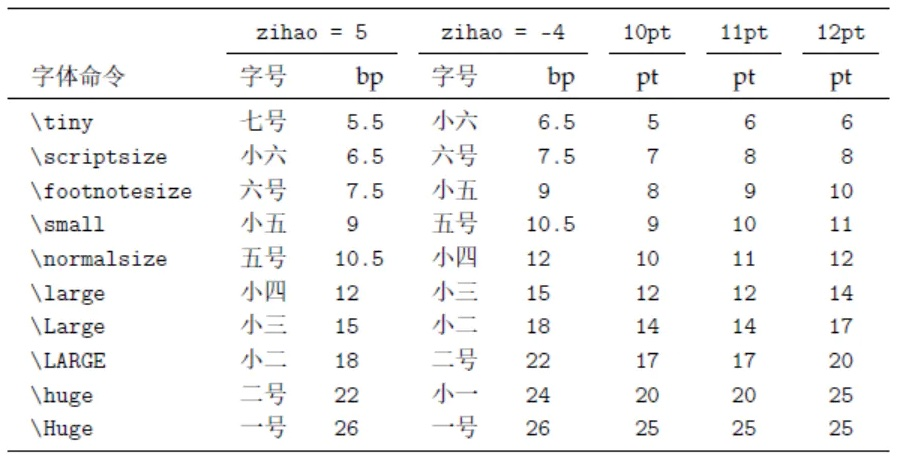
\includegraphics[width=12cm]{zihao.jpg}
	\vspace{5pt}
	\caption{标准字体命令与字号的对应}
	%英文标题begin
	\addtocounter{figure}{-1}
	%\vspace{-5pt}
	%\SetEnglishCaption
	\renewcommand{\figurename}{Figure}
	\caption{Correspondence between standard font commands and font sizes}
	\renewcommand{\figurename}{图}
	%英文标题end
	\label{fig-cor-font}
\end{figure}

\section{中英文间距问题}

自动加入间距. 不再需要在公式、英文前后加字符``\verb|~|''或空格。

\section{引用的问题}


\subsection{参考文献的引用}
参考文献的引用, 用命令~\verb|\cite{ }|. 大括号内要填入的字串, 是自命名的文献条目名。

比如, 通常我们会说:

{\kaishu
	关于此问题, 请参见文献 \cite{CNNIC202249}. 作者某某还提到了某某概念\upcite{林耘森箫2019基于}.}


上文使用的源文件为:

{\kaishu
	关于此问题, 请参见文献~\verb|\cite{CNNIC202249}|. 作者某某还提到了某某概念~\verb|\upcite{林耘森箫2019基于}|.
}

其中~\verb|\upcite| 是自定义命令, 使文献引用呈现为上标形式。

({\heiti 注意:} {\kaishu 这里文献的引用, 有时需要以上标形式出现, 有时需要作为正文文字出现, 为什么?})

另外, 要得到形如~\cite{广西壮族自治区林业厅1993广西自然保护区,du2016overview,2018SYSTEMS,陈俊2020基于} 的参考文献连续引用, 需要用到 cite 宏包(模板已经加入),
在正文中使用~\verb|\cite{r3,r4,r5,r6}| 的引用形式即可.
或者, 连续引用的上标形式: 使用~\verb|\upcite{r1,r2,r5}|, 得到\upcite{CNNIC202249,林耘森箫2019基于,2018SYSTEMS}.

\subsection{参考文献的格式}
模版已经设置好了gbt7714引用格式,默认引用BIBbase格式下的Test-bibtex.bib文件,

在Google Scholar或百度学术找到要引用的文献后点击"引用"然后点击“BibTeX”,复制到bib文件中即可。

中文文献应手动添加一条内容:language = {zh},具体可参考给出的示例文件。

注意,对于专利文件,百度学术引用的文件类型要手动改为~patent。对于会议文件,~booktitle选项应该补上前缀~Proceedings of


\subsection{定理和公式的引用}

\begin{theorem}[谁发现的]\label{th-abcd}
	最大的正整数是~$1$.
\end{theorem}

\begin{proof}
	要找到这个最大的正整数, 我们设最大的正整数为~$x$, 则~$x \geqslant 1$, 两边同时乘以~$x$, 得到
	\begin{equation}\label{eq-abc}
		x^2 \geqslant x.
	\end{equation}
	而~$x$ 是最大的正整数, 由~\eqref{eq-abc} 式得到
	\[
	x^2 = x.
	\]
	所以
	\begin{equation*}
		x = 1.
	\end{equation*}
\end{proof}

定理~\ref{th-abcd} 是一个重大的发现.

%%%%----- 定义等环境的举例 --------
\begin{definition}[整数]
	正整数(例如 1, 2, 3)、负整数(例如 ${−1}$, $−2$, $−3$)与零(0)合起来统称为{\heiti 整数}.
\end{definition}

\begin{remark}
	整数集合在数学上通常表示为 $\mathbf{Z}$ 或 $\mathbb{Z}$, 该记号源于德语单词 Zahlen(意为``数'')的首字母.
\end{remark}

\begin{proposition}
	任意两个整数相加、相减、相乘的结果, 仍然是整数.
\end{proposition}

\begin{example}
	$1+2=3$.
\end{example}

\begin{corollary}
	在整数集合内, 相加、相减、相乘运算是封闭的.
\end{corollary}

\section{图形与表格}

支持 eps, pdf, jpg 这几种常见图形格式.

再次澄清一个误会: \LaTeX{} 支持的图形格式绝非 eps 这一种. 无需特意把图片转化为 eps 格式.

用形如 \verb|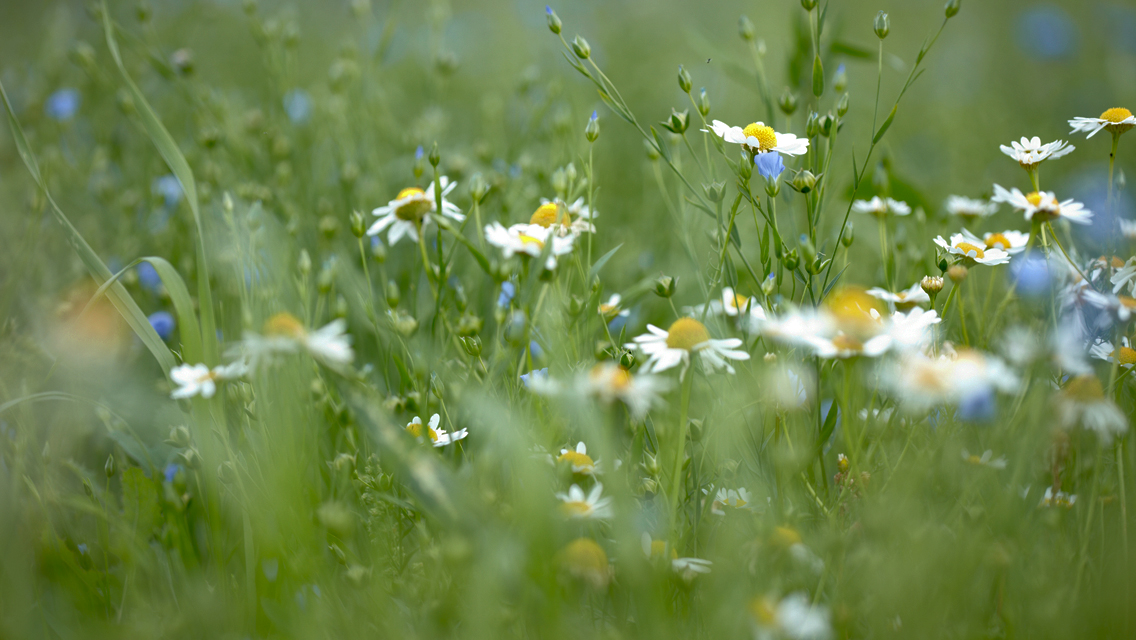
\includegraphics[width=12cm]{Daisy.jpg}| 的命令可以纳入图片.

如图 \ref{fig:1} 是一个纳入~jpg 图片的例子,已经按要求做了中英文双行标题。

\begin{figure}[ht]
	\centering
	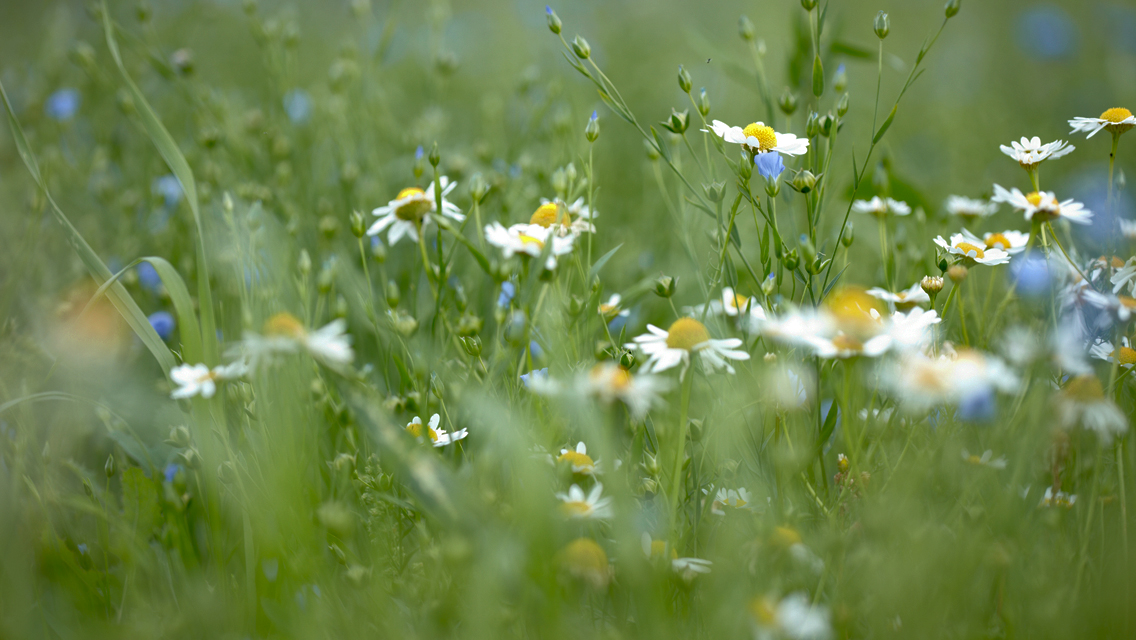
\includegraphics[width=\textwidth]{Daisy.jpg}
	\vspace{1pt}
	\caption{一个彩色 jpg 图片的例子}
	%英文标题begin
	\addtocounter{figure}{-1}
	%\vspace{-5pt}
	%\SetEnglishCaption
	\renewcommand{\figurename}{Figure}
	\caption{An example of a color jpg image}
	\renewcommand{\figurename}{图}
	%英文标题end
	\label{fig:1}
\end{figure}

表格问题, 建议使用``三线表'', 如表 \ref{tab:1}.

\begin{table}[ht]
	\centering
	\caption{一般三线表}
	%英文标题begin
	\addtocounter{table}{-1}
	%\SetEnglishCaption
	\renewcommand{\tablename}{Table}
	\caption{General three-line table}
	\renewcommand{\tablename}{表}
	%英文标题end
	\vspace{2pt}
	\label{tab:1}
	\begin{tabular}{c c c c c c c c c c c}
		\hline
		123 & 4  & 5  & 123 & 4 & 5123 & 4 & 5 & 123 & 4 & 5\\
		\hline
		67 & 890 & 13 & 123 & 4 & 5123 & 4 & 5 & 123 & 4 & 5\\
		67 & 890 & 13 & 123 & 4 & 5123 & 4 & 5 & 123 & 4 & 5\\
		67 & 890 & 13 & 123 & 4 & 5123 & 4 & 5 & 123 & 4 & 5\\
		\hline
	\end{tabular}
\end{table}

此外,还可以插入子图,,引用时效果图~\ref{fig-subfigure},第2张子图可使用图~\ref{fig-subfigure}\subref{fig-subfigure2}进行引用,排版通过控制子图宽度控制。

\begin{figure}[H]
	\centering
	\subfigure{\label{fig-subfigure1}}\addtocounter{subfigure}{-2}\subfigure[Subfigure1]{\subfigure[子图1]{
			
\includegraphics[width=6cm]{Subfigure1.jpg}
	}}
	\quad
	\subfigure{\label{fig-subfigure2}}\addtocounter{subfigure}{-2}\subfigure[Subfigure2]{\subfigure[子图2]{
			
\includegraphics[width=6cm]{Subfigure2.jpg}
	}}
	\subfigure{\label{fig-subfigure3}}\addtocounter{subfigure}{-2}\subfigure[Subfigure3]{\subfigure[子图3]{
			
\includegraphics[width=6cm]{Subfigure3.jpg}
	}}
	\subfigure{\label{fig-subfigure4}}\addtocounter{subfigure}{-2}\subfigure[Subfigure4]{\subfigure[子图4]{
			
\includegraphics[width=6cm]{Subfigure4.jpg}
	}}
	\caption{子图的使用}
	%英文标题begin
	\addtocounter{figure}{-1}
	%\vspace{-5pt}
	%\SetEnglishCaption
	\renewcommand{\figurename}{Figure}
	\caption{Use of subgraphs}
	\renewcommand{\figurename}{图}
	%英文标题endmod-str
	\label{fig-subfigure}
\end{figure}

\section{算法写法}

算法的书写使用\verb|breakablealgorithm|环境,该自定义环境使得算法支持跨页(不再使用\verb|\begin{table}[htbp]|控制定位),效果如下:
\begin{breakablealgorithm}%[h]
	\caption{ 算法示例} 
	\label{alg:flow-table-del} 
	%\resizebox{.95\columnwidth}{!}{
		\begin{algorithmic}[1] %这个1 表示每一行都显示数字
			\Require 第一个输入$a$\Comment{注释这么写}\newline 第2个输入$b$  \Comment{这么换行}%算法的输入参数:Input
			\Ensure 输出$y$	%算法的输出:Output
			\If{ a>b} 
			\State 结果
			\Else
			\While {a<b}
			\State 内容
			\EndWhile
			\EndIf
			\State \Return $y$%算法的返回值
		\end{algorithmic}
		%}
\end{breakablealgorithm}

\section{手动排版}

对于图片和表格,一般使用形如\verb|\begin{figure}[ht]| 、\verb|\begin{table}[ht]|进行自动排版,即优先在上下文位置,如果放不下则插在其他页顶。如果需要强制在当前位置,可以将\verb|[ht]| 改为\verb|[H]| 
		
此外,形如\verb|\vspace{2pt}|也可以用于灵活调整排版,用于手动修正。

\chapter{论文提交}

一般来说提交论文共(给导师)、盲审、(打印)答辩、图书馆四个版本。

当前版本下,盲审时注意编译模版隐去个人信息。


\section*{电子版论文提交}

进入研究生论文提交系统(\url{http://xwlw.lib.njtech.edu.cn/changeMain.action})点击``论文提交'', 进入论文提交系统。
论文提交成功的 3 个工作日后, 可前往图书馆办理离校手续。


\section*{纸本论文提交}

电子版论文提交审核通过的, 请提交 1 份纸本论文到相应的论文纸本进学位档案,记得导师签字。

%%%=== 参考文献 ========%%%
\phantomsection
\addcontentsline{toc}{chapter}{参考文献}
\zihao{5}%参考文献用五号字
\bibliography{BIBbase/Test-bibtex}

\ifprint
\cleardoublepage 
\fi

\normalsize%后面的奖项、致谢恢复小四号字
\backmatter
% !Mode:: "TeX:UTF-8"

%%% 此部分内容:  (1) 攻读硕士学位期间参加的科研项目  (2) 攻读硕士学位期间完成的学术成果  (3) 攻读硕士学位期间获得的奖项  (4) 致谢

%%%=== 攻读硕士学位期间参加的科研项目 ========%%%
\project
\thispagestyle{onlytitle}
\begin{enumerate}[{[1]}]
	\item   国家自然科学基金项目“链路相关无线网络中基于网络编码的数据分发机制研究”(项目编号:61502230);
\end{enumerate}


%%%=== 攻读硕士学位期间完成的学术成果 ========%%%
\achievement
\thispagestyle{onlytitle}
 \textbf{【本人或者导师作为第一作者文章】}
\begin{enumerate}[{[1]}]
	\item   \textbf{Yiren Gu(顾伊人)}, Hang Shen, Guangwei Bai, Tianjing Wang, Xuejun Liu. QoI-Aware Incentive for Multimedia Crowdsensing Enabled Learning System[J], Multimedia Systems (Springer), 2020, 26(1): 3-16, DOI 10.1007/s00530-019-006 16-w (SCI,中科院三区,CCF推荐C类期刊,篇幅14页)
	\item 国家发明专利:一种用于机器学习系统的多媒体群智感知激励方法,发明人:白光伟,\textbf{顾伊人},沈航,沙鑫磊,张杰,申请号:201910096432.X,申请日期:2019年1月31日,已受理 (第二发明人,导师为第一发明人)
\end{enumerate}
\par
 \textbf{【合作发表成果】}
\begin{enumerate}[{[1]}]
	\item   国家发明专利:一种数据质量感知的移动群智感知激励方法, 发明人:白光伟, 童海, 沈航, \textbf{顾伊人}, 胡煜家,申请号: 201910455446.6,申请日期: 2019年 05 月 29 日,已受理
\end{enumerate}


%%%=== 攻读硕士学位期间获得的奖项 ========%%%
\awards
\thispagestyle{onlytitle}
\textbf{【本人或者导师作为第一作者文章】}
\begin{enumerate}[{[1]}]
	\item 2019年12月获2019年度“硕士研究生国家奖学金”;
	\item 2019年12月评为2019年度计算机科学与技术学院“优秀共产党员”;
	\item 2019年9月评为计算机科学与技术学业“优秀部长”;
	\item 2019年9月获校研究生学业奖学金特等奖;
\end{enumerate}

%%%%%%%%%%%%%%%%%%%%%%%
%%% --------------- 致谢 ------------- - %%%
%%%%%%%%%%%%%%%%%%%%%%%
\acknowledgement
\thispagestyle{onlytitle}

感谢你, 感谢他和她, 感谢大家.

%%%%%%%%%%%%%%%%%%%%%%%%%%%%%%%%%%%%%%%
%%%%%%%--判断是否需要空白页-----------------------------
  \iflib
  \else
  \newpage
  \cleardoublepage
  \fi
%%%%%%%-------------------------------------------------







 %%%攻读硕士学位期间参加的科研项目,学术成果,奖项,致谢.
%\cleardoublepage
\end{document}




